\chapter{Covariate modeling}

As I have mentioned frequently in previous sections, the
epidemiological data on disease morbidity collected in systematic
review is often very sparse and very noisy.

Covariate modeling is a method to \emph{explain} the noise in noisy
data in terms of demographic, epidemiological, and study-specific
variables.  This is often challenging because there is no particularl
explanatory variable available, and also because the data are very
sparse.  Nonetheless, this approach has a long history of relevant
application, in global health and
economics. \cite{Girosi_Demographic_2008,Wakefield_Bayesian_1996} TK
connections to and references from this work, possibly including the
work of Gary King's Book on demographic forecasting, Andrew
Gelman's work, some tradition of macroeconomics which I need to learn
more about, Jon Wakefield's covariate modeling in PK paper,
references therein.

In the integrative systems model of disease in populations, covariate
modeling has two distinct goals.  First, covariates are a way to
explain the bias and variation of the noisy measurements of
epidemiological rates.  And second, covariates are a way to increase
the accuracy of out-of-sample predictions.  This is accomplished by
modeling the relationships between the disease parameters of interest
and the explanatory covariates. The modeled relationships are then
used to extrapolate predictions for the disease parameters to
geographic regions where covariate data is available, but no direct
measurements are made.

In covariate modeling, there is often a distinction made between
``fixed effects'' and ``random effects''.  Bayesian approaches, such
as hierarchical modeling, blur this distinction (to the point that
hierarchical modeling is also called ``mixed effect'' modeling
\cite{Gelman_Multilevel_2005}.  To make the nomenclature more
complicated, different methodological traditions of covariate modeling
have opposite concepts of what is fixed and what is random in effects.

For integrative systems models of disease, I make the following
explicit distinction between fixed effects and random effects: while
fixed effects may take any value, random effects are constrained to
sum to zero.  Although there is no standard meaning of random effect
in interdisciplinary research, this approach that I have taken, and
will elaborate on below, seems to be particularly non-standard.
However, as I will argue, it is quite appropriate and convenient in
this setting.

TK bridge paragraph describing the order and contents of the coming
sections.
\section{Fixed effects to explain bias}

A prototypical example comes from myocardial infarction (MI)
incidence, where there are a variety of diagnostic tests available and
different studies of IHD prevalence use different diagnostic criteria
for case ascertainment.  The newer class of tests, which are based on
measuring levels of the blood protein troponin, are more sensitive
than earlier methods, and this leads to variation in data with a clear
explanation.  Figure~\ref{cov-sim} shows simulated data with a
covariate that has an effect like a troponin-based test might, raising
the number of observed cases by 30\%. By including an indicator
variable as a covariate in each row of data, $x_i = 1$ if row $i$
comes from a study that used a troponin test, and $x_i = 0$ otherwise,
I can fit a model which includes a parameter to ``cross-walk'' between
studies using these two different case ascertainment criteria.

\begin{figure}[h]
\begin{center}
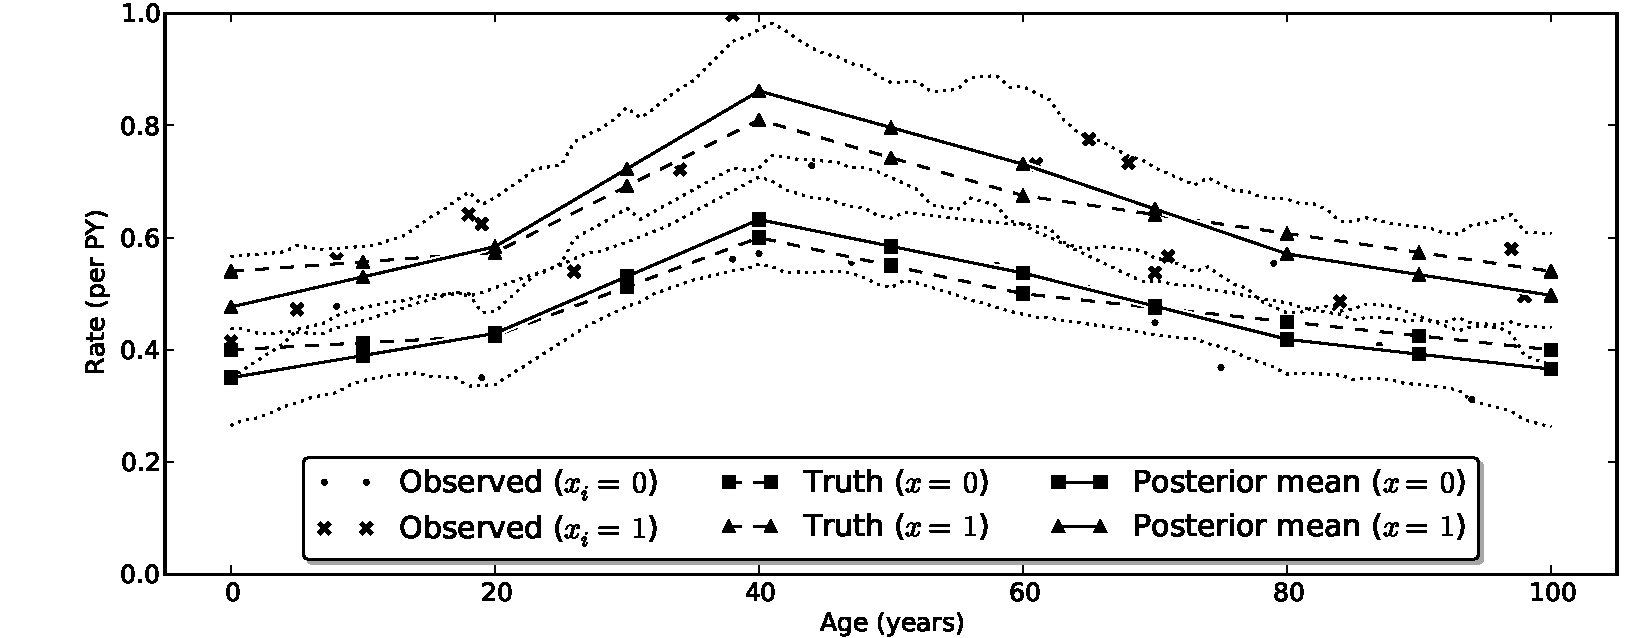
\includegraphics[width=\textwidth]{cov_fe.pdf}
\caption{TK description of covariate model, data with $x_i=1$ are on average 30\% higher than data with $x_i=0$.}
\label{cov-sim}
\end{center}
\end{figure}

TK This same approach can be applied to questions with varying
duration that come up in the meta-analysis of psychological disorders,
for example anxiety disorder is sometimes measured in past month
prevalence and sometimes in past year prevalence.

TK In addition to dichotomous variables, like diagnostic criteria or
bias, covariate modeling can be applied to continuous covariates, like
GDP, Animal Fat consumption, PfPR, or anything.  An example which uses
covariates derived from the country where the study took place is in
MS.  Here experts believe that there is a correlation between disease
prevalence and distance from the equator.  By including the absolute
value of latitude (normalized over all countries to have mean 0 and
variance 1), the model is able to reduce the variance slightly. TK
another example of how covariates can explain some of this variation
is cirrhosis prevalence; in Europe data variation is explained by
alcohol consumption per capita.


In general, let the data collected in systematic review be denoted by
tuples $\left(a_i, n_i, r_i, X_i\right)$, where $a_i$ is the age
group, $n_i$ is the effective sample size, $r_i$ is the observed rate
value, and $X_i$ is a vector of covariate values. The fixed-effect
covariate model is then the following:
\begin{align*}
r_i, n_i &\sim \NBRate\left(\mu_i, \delta\right),\\
\mu_i &= \boldmu(a_i)e^{\beta X_i}
\end{align*}

The parameter $\beta$ represents the effect coefficients for
the fixed effects, and because the data is often sparse and noisy, it
can help the stability of the computational algorithms to put a weakly
informative prior on $\beta$, such as
\[
\beta_j \sim \Normal\left(0, 1^2\right) \text{ for } j = 1, \ldots, J.
\]
Of course, if experts have beliefs about the sign or magnitude of the
effect coefficient, this can be included as a more informative prior.

Two subtle choices are worth additional investigation in fixed effect
modeling: reference values and normalization.  Both of these choices
are known to influence the performance of computational
algorithms. For example, non-normalized covariates can produce
non-convergence in hill-climbing algorithms that work fine with
normalized covariates.  But because of the Bayesian priors and
especially because of the consistency from the compartmental model,
the choices are particularly important in this setting.

The term \emph{reference value} is borrowed from fixed effects
modeling of categorical variables, where so-called dummy variables
(zero/one indicators) are introduced for all but one category. When
all the dummy covariates are set to zero, the model produces
predictions for the reference category. In the formulation above, the
analogous notion occurs when $X_i = (0, 0, \ldots, 0)$.  Then the
expression for $\mu_i$ simplifies to
\[
\mu_i = \boldmu(a_i) e^{\beta \0} = \boldmu(a_i).
\]
It is this $\boldmu$ that is used as the age-specific rate function in
the compartmental model (as developed in
Chapter~\ref{theory-system_dynamics}), so the consistency between
incidence, prevalence, remission, and mortality is enforced at the
reference values.

Because the reference values are consistent, they must be chosen with
care.  For example, in the case of IHD above, where some studies used
troponin based diagnostics and some did not, the reference value
should be \emph{with} troponin tests, because this is considered to be
much more accurate.

TK example, with graphic of the effects of different reference values
(on real or synthetic data)

Normalization is also important, although it does not affect
consistency.  It is important for stability of numerical algorithms,
and also because the prior on the effect coefficient must be matched
to the scale of the covariate.  Normalizing continuous covariates to
have variance one, for example, means that the prior of
$\beta\sim\Normal(0,1^2)$ is weakly informative.  If a continuous
covariate had variance $0.0001$, the same prior on $\beta$ would be
very informative.

\section{Fixed effects to explain variation}
TK transition paragraph, it is also possible to use fixed effect
covariate modeling to explain the different levels of variation in
different sources of data.

TK cleaned up version of the following example that leads to the same
mathematical model deals with studies that target specific
populations.  For example, systematic review led to collecting a
number of Hepatitis C prevalence studies that used voluntary blood
donors as the sample frame.  This is clearly not the whole population,
but it is not obviously a biased sample.  It all depends on whether
the people who volunteer to give blood have a higher or lower
prevalence of Hepatitis C than the general population. Disease experts
believe that \emph{paid} blood donors are not representative of the
general population, but do not have a strong prior belief about the
representativeness of voluntary donors.  This is another place where
covariate approach is appropriate. In the Hepatitis C example (to be
elaborated on in Chapter~\ref{TK}), the systematic review coded rows
corresponding these voluntary blood donors, as well as other studies
of specific subpopulations, such as mothers visiting antenatal
clinics, with a bias indicator $z_i = 1$, and coded rows from studies
of the general population with $z_i = 0$.  In this case it is
appropriate to introduce a parameter for the bias introduced by
sampling from these subpopulations, but it is also appropriate to
introduce a parameter for these variables to have over-dispersion that
differs from the studies of the general population.

This \emph{generalized negative binomial model} has the following
formulation:
\begin{align*}
r_i, n_i &\sim \NBRate\left(\mu_i, \delta_i\right),\\
\mu_i &= \boldmu(a_i)e^{\beta X_i},\\
\delta_i &= e^{\eta + \zeta Z_i}.
\end{align*}

TK figure showing with and without this approach, or possibly a range
of priors on zeta.


\section{Fixed effects models are not causal models}
TK a discussion of the inappropriateness of using this for causal
analysis, as well as a recognition that people are going to be really,
really tempted to.

Additional covariates to consider: conflict for anxiety, PTSD. Health
system access for AF.  Ask Theo what else has been popular.

Include examples of unexpected direct of effects, colinearity leading
to distinctly non-causal conclusions, etc.

\section{Random effects for unexplained variation}
Another important use of covariates is in handling non-sampling
variation that \emph{cannot} be explained. As I have mentioned
repeatedly, the descriptive epidemiological data available is often
very noisy.  It is usually only a small part of this ``noise''
that can be explained with covariates like those from the preceding
section. And while the additional variation has no simple explanation
in terms of differing diagnostic criteria or the like, there is
structure in the variation. Countries in the North Africa/Middle East
region have rates more similar to each other than to countries in the
North America, High Income region.  And the North America, High Income
region as a whole is more similar to the Europe, Western region than
to the Asia, South region.  These spatial similarities are a candidate
for random effects modeling.

I will develop this approach to random effects modeling by beginning
with something very similar to the fixed-effects model, and then
constraining the parameters to have certain sums equal to zero.  For
notation, let $U_i$ be a vector of random effect covariates.  This
$U_i$ is a \emph{design matrix} analogous to the fixed-effect
covariate vector $X_i$ above, but with zero/one values corresponding
to the place in the spatial hierarchy to which observation $i$ refers.

In GBD 2010, the spatial hierarchy is countries nested in regions
nested in super-regions, but in national or sub-national analyses, the
hierarchy will be different. This can be generically formulated using
graph theory, where a directed tree (also known as an
\emph{out-arborescence}) encodes the hierarchical relationship
structure, with a root node connected by out-arcs to children on the
first level of the hierarchy, which are each in turn connected by
out-arcs to children on the next level of the hierarchy, and so on.  A
node is called the \emph{parent} of any node it points to in this
tree, and two nodes are called \emph{siblings} if they share the same
parent.


Analogously to the fixed effect model above, the random effects apply
a multiplicative shift to the age-specific rate function:
\begin{align*}
r_i, n_i &\sim \NBRate\left(\mu_i, \delta_i\right),\\
\mu_i &= \boldmu(a_i)e^{\alpha U_i}.
\end{align*}
The first difference between the fixed effects and random effects is
in the priors on the effect coefficients.  Instead of a weakly
informative prior as above, the prior on $\alpha$ is itself part of
the model, parameterized as:
\[
\alpha_j \sim \Normal\left(0, \sigma_{\ell(j)}^2\right),
\]
where $\ell(j)$ is the level in the hierarchy of node $j$, and
$\sigma_\ell$ is also a model parameter. To fit this model with
Bayesian methods, we also need a prior on $\sigma_\ell$ (a
hyper-prior), and because of the sparse and noisy nature of the
available data, this often has to be somewhat informative.  The
truncated normal distribution
\[
\sigma_\ell \sim \Normal_{[.05,5]}\left(.05, .03^2\right),
\]
is often an appropriate choice. It says that between-area variation of
less than 5\% is impossible and more than 15\% is rare.

The second difference between the fixed effects and random effects is
the following: for every node in the spatial hierarchy, the random
effects for all children of that node must sum to zero.  And if there
is no data for some node, its random effect must be zero.  This
captures the modeling philosophy that random effects represent
unexplained, but true, variation of nodes in the area hierarchy from
the central tendency of their siblings.  Using $H$ to denote the
hierarchy, this constraint can be formalized mathematically as
\begin{align*}
\sum_{c\in N^+(p)} \alpha_c &= 0, \text{ for all } p \in N;\\
\alpha_c &=0, \text{ for all $c$ such that } \sum_{i} U_i(c) = 0.
\end{align*}

Some examples will make this clearer.  TK examples, with a figure
showing maps that exhibit spatial similarity.

\section{Covariates to predict out-of-sample}

In addition to explaining, or at least quantifying, the noise in the
noisy data, covariate modeling can help in predicting levels for the
times and places which the sparse data does not cover.  This
\emph{out-of-sample prediction} works by borrowing strength between
regions, sexes, and times, as well as leveraging the consistency
conditions formalized by the compartmental model.  But it works better
when there is a relationship between the disease parameters of
interest and some covariate or covariates for which the values are
known for that time and place.

TK An example comes from modeling the incidence of Liver Cancer.
Although there is no data on much of the world, there is data on hep
c, and this can be used as a covariate.  smoking and copd? Etc.

TK Some evidence (from simulation study?) that it is a good idea would
be nice to present as well.

TK paragraph on aggregating predictions for the lowest level of the
hierarchy into regional values.  country-specific values, and how they
are aggregated into regional estimates - fixed reference value

TK paragraph on using $\sigma_\ell$ to ``know how much we know''
when there is a region with data from one country only.

\section{Covariates and consistency}
One of the most challenging theoretical issues in covariate modeling
for integrative systems modeling is the interplay between the
predictive covariates and the inter-compartmental consistency.  A
simple example of the problem arises in a model of congenital
abnormalities, where there is birth prevalence, but no incidence or
remission, and data on prevalence and cause-specific population
mortality. If covariates are used to shift predictions for the level
of $pf$ as well as the level of $p$ and the level of $f$, then
consistency would require that $\beta^{pf}_i = \beta^p_i + \beta^f_i$.

This complication becomes even more pronounced in a model where there
is non-zero incidence and remission.  In the general case, it is not
even clear that non-zero covariate effects \emph{exist} which respect
consistency.

To circumvent this challenge, I have used a multistage approach to
fitting the model (see Section~\ref{empirical-priors}), and at each
stage of the process, there is a specific level of the hierarchical
model where I have enforced the consistency conditions of the system
dynamics model.  All predictions from this stage apply only to this
node and nodes lower in the hierarchy, and for the lower nodes, the
predictions are \emph{not} consistent.  However, they are expected to
be \emph{close to consistent}, a hypothesis that must be investigated
empirically on a case-by-case basis.

How does this work?  Recall the covariate model formulation for
predicting the rate for a given area, sex, and year $(a,s,y)$,
\[
\boldpi_{a,s,y}(a) = \boldmu(a)e^{\alpha U_{a,s,y} + \beta X_{a,s,y}}. 
\]
For the highest node of the hierarchy (also called the
\emph{reference} node, and corresponding to area/sex/year $(a_r, s_r,
y_r)$), I simply apply a linear shift to each covariate in $X$ and $U$
to have $X_{{a_r},{s_r},{y_r}} = \0$ and $U_{a_r,s_r,y_r} = \0$.  This
yields \[ \boldpi_{a_r,s_r,y_r}(a) = \boldmu(a), \] and for any system
of differential equations that $\{\boldmu^t(a), t=[T]\}$ are
solutions, the predicted values for the age, sex, year at the root of
the hierarchy are also solutions.

An important direction for future work is to go beyond the multistage
approach.  This will probably require innovation in algorithms,
because fitting multiple consistent models simultaneously is currently
impractical.

\section{Identifiability}
The random effects modeling approach described above must be
implemented with caution.  In a naive implementation, the effects at
the super-region, region, and country level will interact in a way
that leads to ``non-identifiability''.  While this is not a
theoretical limitation in the Bayesian framework, it has practical
ramifications: the MCMC algorithm will not converge well when there
are many random effects that can all do the same job.  To avoid this,
it is important to choose which area random effects to include
carefully.

For this reason, a random effect for area $a$ is only included in the
model if the likelihood includes data for descendants of at least two
distinct children of $a$.

TK additional discussion of this, possibly examples

\section{Hyperpriors}
TK The priors on the random effects have a large impact on the
estimates as well, and a theoretically grounded selection of these
effects is crucial.  I have used a default hyperprior on the standard
error of the random effect, chosen from a weakly informative
distribution TK, $\sigma_{\alpha_i} \sim \Uniform[.0005, .05]$.  The
structure of these hyperpriors is important as well, and I have use a
TK common $\sigma_{\alpha_i}$ for all random effects at the same level
of the area hierarchy.  This operationalizes an assumption that the
unexplained systematic variation between children of a node in the
area hierarchy is the same for all sets of children on the same level.
For example, the unexplained systematic variation between the regions
in the sub-Saharan Africa super-region is assumed to be the same that
the unexplained systematic variation between regions in the Latin
America super-region.

\section{Co-linearity}
TK Choosing co-linear covariates for the fixed effects leads to bad
convergence and unpredictable results.  Care must be taken to avoid
this, and cirrhosis data give an example of how things can go wrong if
cirrhosis CSMR and alcohol consumption are both included as
``country-level covariates''.

\section{Simulation}
TK This section describes a simulation study designed to confirm that
the covariate model performs as expected.  It also serves as a
validation of the implementation of the covariate model, which is the
most complicated part of the model to implement and hence the most
prone to error.

The simulation approach is as follows:
\begin{enumerate}
\item Choose a true prevalence value $p^\true$ uniformly at random
  from the interval $(.0001, .1)$
\item Choose true random effect dispersion values $\sigma_\ell^\true$
  uniformly at random from $(.05, 5)$ \item Choose true random effect
  values $\alpha_a$ from the normal distribution with standard
  deviation $\sigma_{\ell_a}$, where $\ell_a$ is the level of area $a$
  in the spatial hierarchy.
\item Generate $N$ observations, $p_1,\ldots,p_N$ by choosing an area
  $a_i$ uniformly at random from the area hierarchy and an effective
  sample size $n_i$ uniformly from $[100,10000]$, and then using a
  negative binomial distribution to select $p_i \sim
  \NegativeBinomial(n_i p^\true_{a_i}, \delta n_i
  p^\true_{a_i})/n_i$.
\end{enumerate}

This provides a simulation dataset for testing the performance of the
random effects covariate model when there is no specification
error. It is useful for understanding the relationship between data
sparsity and data error and estimation accuracy, as well as for
testing the implementation of the model.

There is one complication here, which I'm not sure how to deal with,
and that is the model assumes that the random effects sum to zero for
all of the countries with data in a region (or all the regions with
data in a super-region).  This is approximately true in the simulation
scheme above, because in expectation the random effects sum to zero,
and as the number of countries in a region grows large, the
realization quickly approaches its expectation.  It is quite untrue in
certain regions, however, because there actually are not many
countries.  For example, the North America, High Income region has
only two countries, USA and Canada.

A simple fix is to violate the distributional assumption, and replace
one of the country random effects in each region with the appropriate
value to make them all sum to zero.  This matches the model
implementation pretty well.

